% MODIFICA EL CONTENIDO QUE VIENE A CONTINUACIÓN DE ACUERDO A TU TRABAJO

\chapter{Problema del Bandido de $k$-brazos}

%%%%%%%%%%%%%%%%%%%%%%%%%%%%%%%%%%%%%%%%%%%%%%%%%%%%%%%%%%%%%
%%%%%%%%%%%%%%%%%%%%%%%%%%%%%%%%%%%%%%%%%%%%%%%%%%%%%%%%%%%%%
\section{Introducción }

En varios aspectos de la vida cotidiana un agente debe tomar decisiones repetidas bajo incertidumbre con el objetivo de maximizar su beneficio acumulado: selección de tratamientos médicos, personalización de contenidos en portales digitales... El \textbf{problema del bandido multibrazo} (o de k-brazos) es un escenario clásico para la aplicación de aprendizaje por refuerzo \cite{robbins1952} que captura y modela matemáticamente este tipo de problema. El paradigma
planteado es un agente que debe seleccionar secuencialmente acciones (brazos) de extracción para maximizar las recompensas acumuladas a lo largo del tiempo.
Se asume que las diferentes recompensas siguen distribuciones de
probabilidad ocultas y que el resultado de cada acción es independiente
de las anteriores. 

El agente puede almacenar en cada instante diferentes estadísticos que guíen
sus futuras elecciones. Según su método de toma de decisiones, distinguimos dos
comportamientos:

\begin{itemize}
    \item \textbf{Exploración}: el agente selecciona un brazo (no necesariamente el óptimo)
    para aumentar su información sobre el mismo y aprovechar el nuevo dato para reforzar sus 
    estadísticos. Un comportamiento puramente exploratorio obtiene una recompensa media igual a
    la media de las recompensas individuales de los brazos.
    \item \textbf{Explotación}: el agente selecciona el brazo que considera que ofrece mejores
    recompensas. Esta selección se hace en general según la media. Un comportamiento puramente 
    explotador obtendrá una recompensa media igual a la media de uno de los brazos. Dependiendo
    de las elecciones iniciales, es posible que este brazo no sea el óptimo.
\end{itemize}

El \textbf{Dilema Exploración-Explotación} es el núcleo central del problema y todos los algoritmos que se plantean en este paradigma tratan de forma diferente de llegar a un equilibrio que maximice
las recompensas en un horizonte temporal indeterminado.

En este capítulo comparamos tres familias de algoritmos (\textbf{$\epsilon$-\textit{greedy}}, \textbf{UCB} y \textbf{\textit{Softmax}}) sobre tres bandidos con distribuciones de
probabilidad diferentes (\textbf{Bernoulli}, \textbf{binomial} y \textbf{normal}), con el objetivo de determinar los mejores agentes para cada problema o 
comprobar si existe algún método claramente superior a los demás en todos los escenarios.

El capítulo se organiza presentando primero la definición formal del problema y las métricas empleadas, seguido de los pseudocódigos de cada algoritmo, los resultados experimentales para cada tipo de bandido, y finalmente las conclusiones del estudio.

Todo el código desarrollado en este apartado se puede encontrar en el repositorio de GitHub \href{https://github.com/rafelsalgueiro/GallegoSalgueiroVera}{https://github.com/rafelsalgueiro/GallegoSalgueiroVera}. El esqueleto del mismo ha sido proporcionado por el profesor de la asignatura. Los experimentos han sido desarrollados en los \textit{notebooks} que se encuentran dentro de la carpeta `k\_brazos'.

\section{Desarrollo}

El problema se enmarca como un proceso de toma de decisiones secuencial donde un agente interactúa con un entorno compuesto por múltiples opciones independientes. Sea $t$ un instante de tiempo dado y $\mathcal{A}=\{1,...,K\}$ el conjunto de las posibles acciones. Definimos: 

\begin{itemize}
    \item Acción: $A_t\in \mathcal{A}$.
    \item Recompensa: $R_t\in \mathbb{R}$.
\end{itemize}

Cada acción $a$ tiene asociada una recompensa esperada que llamaremos $\mu_a$:
$$\mu_a=\mathbb{E}[R_t \mid A_t=a]$$
El objetivo principal del agente es maximizar la suma total de las recompensas obtenidas a lo 
largo de los $T$ pasos de tiempo. Para formular nuestras métricas es útil definir de antemano el brazo
óptimo y su valor:
\begin{itemize}
    \item Brazo óptimo: $a^*=argmax_a\{\mu_a\}$
    \item Recompensa esperada óptima: $q^*=max_a\{\mu_a\}$
\end{itemize}

Para evaluar qué tan bien funciona una estrategia, utilizamos las siguientes métricas \cite{sutton2018}:

\begin{itemize}
    \item \textbf{Recompensa media acumulada:} el valor esperado de la suma de recompensas hasta el paso $T$. 
    $$\mathbb{E}\left[\sum^T_{t=1}R_t \right]$$
    \item \textbf{Tasa de elección del brazo óptimo:} la probabilidad de que el algoritmo haya aprendido a seleccionar la mejor acción posible en el instante $T$.
    $$\mathbb{P}\left[A_T=a^* \right]$$
    \item \textbf{Arrepentimiento acumulado:} diferencia entre la recompensa total que el agente habría obtenido si hubiera conocido y elegido siempre el brazo óptimo y la recompensa que obtuvo.
    $$L_T=T\times q^*-\sum^T_{t=1}R_t$$
\end{itemize}

Las tres métricas son complementarias, pero el arrepentimiento acumulado es la más informativa: equivale a medir la distancia entre el comportamiento del agente y el de un agente con conocimiento perfecto que explota siempre el brazo óptimo. Un arrepentimiento que crece sublinealmente con $T$ indica que el agente está aprendiendo de forma efectiva. La \textbf{cota de Lai-Robbins} \cite{lai1985} establece un límite inferior teórico sobre el arrepentimiento acumulado esperado. Formalmente, para un horizonte temporal $T$ suficientemente grande, ningún algoritmo puede hacer mejor que 
$$\mathbb{E}[L_T]\geq \sum_{a: \mu_a < \mu^*}\frac{\mu^*-\mu_a}{KL(\mu_a||\mu^*)}\cdot \ln T,$$
donde $KL(\mu_a||\mu^*)$ es la divergencia de Kullback-Leibler entre la distribución del brazo $a$ y la del brazo óptimo, que mide cuán difíciles son de distinguir estadísticamente. Esta expresión implica que el arrepentimiento de cualquier algoritmo razonable crece al menos de forma logarítmica con el número de pasos. En la práctica, utilizamos esta cota como referencia visual en las gráficas de arrepentimiento acumulado para valorar cuán cerca están los algoritmos evaluados del comportamiento asintóticamente óptimo. 

Por último, los tres tipos de bandidos estudiados se diferencian en la distribución de probabilidad que rige las recompensas de cada brazo:

\begin{itemize}
    \item \textbf{Bandido de Bernoulli:} es el más sencillo. Las recompensas son binarias (0/1) y la recompensa del brazo $a$ sigue una distribución de Bernoulli con un parámetro $p_a \in [0,1]$, que representa la probabilidad de éxito.
    $$R_t\sim Be(p_a)$$
    \item \textbf{Bandido binomial:} las recompensas son discretas ($\{0..n\}$) y la recompensa del brazo $a$ sigue una distribución binomial de $n$ ensayos y probabilidad $p_a$.
    $$R_t \sim Binom(n,p_a)$$
    \item \textbf{Bandido normal:} las recompensas son continuas y la recompensa del brazo $a$ sigue una distribución normal con media $\mu_a$ y desviación típica $\sigma_a$. 
    $$R_t \sim N(\mu_a, \sigma_a)$$
\end{itemize}

Los algoritmos que empleamos están descritos en la siguiente sección \cite{sutton2018}. Al tratarse de una práctica de introducción a un problema clásico, no pretendemos hacer ninguna innovación técnica sino un trabajo exploratorio para comprender mejor estos algoritmos.

%%%%%%%%%%%%%%%%%%%%%%%%%%%%%%%%%%%%%%%%%%%%%%%%%%%%%%%%%%%%%
%\subsection{Trabajos Relacionados}

%Por supuesto puede añadir más subapartados si los necesitara.

%%%%%%%%%%%%%%%%%%%%%%%%%%%%%%%%%%%%%%%%%%%%%%%%%%%%%%%%%%%%%
\section{Algoritmos}

%\begin{itemize}
%    \item Explicar en detalle los pasos de los algoritmos empleados.
%    \item Incluir pseudocódigo y, opcionalmente, diagramas de flujo si es necesario.
%    \item Justificar la elección de los algoritmos y su aplicabilidad al problema estudiado.
%\end{itemize}

\subsection{Familia $\epsilon$-\textit{greedy}}

La primera familia que probamos es la llamada $\epsilon$-\textit{greedy}. En su forma clásica viene controlada por un parámetro $\epsilon\in[0,1]$ que determina la probabilidad de exploración. En el algoritmo~\ref{alg:epsilon_greedy}, en cada elección se decide con una probabilidad $p=\epsilon$ escoger un brazo de forma uniformemente aleatoria (exploración) y con una probabilidad $p=1-\epsilon$ el brazo de mayor valor medio (explotación).

\begin{algorithm}[H]
\caption{$\epsilon$-\textit{greedy}}
\label{alg:epsilon_greedy}
\begin{algorithmic}[1]
\Require $\epsilon \in (0,1)$, $K$, $T$
\State \textbf{Inicialización:}
\For{$a = 1 \dots K$}
    \State $Q(a) \leftarrow 0$ \Comment{Estimación de la recompensa}
    \State $N(a) \leftarrow 0$ \Comment{Contador de elecciones del brazo $a$}
\EndFor
\State \textbf{Interacción con el entorno:}
\For{$t = 1 \dots T$}
    \State $p \leftarrow$ Muestreo $Unif((0,1))$ 
    \If{$p < \epsilon$}
        \State $A_t \leftarrow$ Muestreo $Unif(\{1, \dots, K\})$ \Comment{Exploración}
    \Else
        \State $A_t \leftarrow \arg\max_{a} Q(a)$ \Comment{Explotación}
    \EndIf
    \State $R_t \leftarrow$ Ejecutar $A_t$
    \State \textbf{Actualización de estimaciones:}
    \State $N(A_t) \leftarrow N(A_t) + 1$
    \State $Q(A_t) \leftarrow Q(A_t) + \frac{1}{N(A_t)} \left( R_t - Q(A_t) \right)$
\EndFor
\end{algorithmic}
\end{algorithm}

También empleamos una variante con decaimiento del parámetro $\epsilon$. La motivación es dedicar las iteraciones iniciales a una exploración exhaustiva y reducir progresivamente la aleatoriedad conforme el agente acumula conocimiento, favoreciendo la explotación en fases avanzadas. La actualización de $\epsilon$ sigue la regla $\epsilon_t=\frac{\epsilon_0}{1+\lambda t}$, donde $\lambda>0$ controla la velocidad de decaimiento. 

\begin{algorithm}[H]
\caption{$\epsilon$-\textit{greedy} con decaimiento proporcional}
\label{alg:epsilon_decay}
\begin{algorithmic}[1]
\Require $\epsilon_0 \in (0,1)$, $\lambda>0$ $K$, $T$
\State \textbf{Inicialización:}
\For{$a = 1 \dots K$}
    \State $Q(a) \leftarrow 0$ \Comment{Estimación de la recompensa}
    \State $N(a) \leftarrow 0$ \Comment{Contador de elecciones del
    brazo $a$}
    \State $\epsilon \leftarrow \epsilon_0$
\EndFor
\State \textbf{Interacción con el entorno:}
\For{$t = 1 \dots T$}
    \State $p \leftarrow$ Muestreo $Unif((0,1))$ 
    \If{$p < \epsilon$}
        \State $A_t \leftarrow$ Muestreo $Unif(\{1, \dots, K\})$ \Comment{Exploración}
    \Else
        \State $A_t \leftarrow \arg\max_{a} Q(a)$ \Comment{Explotación}
    \EndIf
    \State $R_t \leftarrow$ Ejecutar $A_t$
    \State \textbf{Actualización de estimaciones:}
    \State $N(A_t) \leftarrow N(A_t) + 1$
    \State $Q(A_t) \leftarrow Q(A_t) + \frac{1}{N(A_t)} \left( R_t - Q(A_t) \right)$
    \State $\epsilon \leftarrow \frac{\epsilon_0}{1+\lambda t}$
\EndFor
\end{algorithmic}
\end{algorithm}

\subsection{UCB}

Esta segunda familia (\textit{Upper Confidence Bound}) introduce el concepto de exploración dirigida basada en el principio de `optimismo frente a la incertidumbre'. En lugar de separar rígidamente las dos fases, UCB1 (algoritmo~\ref{alg:ucb1}) evalúa el potencial de cada brazo como una ponderación del valor estimado y un margen de confianza que representa la incertidumbre acumulada sobre ese brazo. La fórmula de selección es:
$$UCB1(a)=Q(a)+c\sqrt{\frac{\ln t}{N(a)}}$$
El parámetro $c>0$ regula el peso otorgado a la incertidumbre. Un valor alto de $c$ favorece la exploración: brazos poco visitados recibirán puntuaciones UCB elevadas independientemente de su rendimiento observado. Un valor bajo de $c$ concentra la selección en los brazos con mayor valor estimado, priorizando la explotación. A diferencia de $\epsilon$-\textit{greedy}, UCB1 no explora de forma aleatoria sino dirigida, favoreciendo sistemáticamente los brazos sobre los que existe mayor incertidumbre. 

\begin{algorithm}[H]
\caption{Algoritmo UCB1 (Upper Confidence Bound)}
\label{alg:ucb1}
\begin{algorithmic}[1]
\Require $c > 0$ (típicamente $c = \sqrt{2}$), $K$, $T$
\State \textbf{Inicialización:}
\For{$a = 1 \dots K$}
    \State $R_a \leftarrow $ Ejecutar $a$
    \State $Q(a) \leftarrow R_a$  \Comment{Jugar cada brazo una vez}
    \State $N(a) \leftarrow 1$ \Comment{Contador de selecciones del brazo}
\EndFor
\State \textbf{Interacción con el entorno:}
\For{$t = K+1 \dots T$}
    \For{$a = 1 \dots K$}
        \State $UCB(a) \leftarrow Q(a) + c \sqrt{\frac{\ln t}{N(a)}}$
    \EndFor
    \State $A_t \leftarrow \arg\max_{a} UCB(a)$ \Comment{(romper empates al azar)}
    \State $R_t \leftarrow$ Ejecutar $A_t$ 
    \State \textbf{Actualización de estimaciones:}
    \State $N(A_t) \leftarrow N(A_t) + 1$
    \State $Q(A_t) \leftarrow Q(A_t) + \frac{1}{N(A_t)} \left( R_t - Q(A_t) \right)$
\EndFor
\end{algorithmic}
\end{algorithm}
\vspace{-15pt}

\subsection{Familia \textit{Softmax}}

La estrategia \textit{Softmax} (algoritmo~\ref{alg:softmax}) pondera las probabilidades de exploración según las estimaciones de recompensa actuales \cite{luce1959}. En lugar de elegir siempre la mejor acción, su elección se basa en una distribución de probabilidad dada por la función \textit{Softmax}. Esta probabilidad viene controlada por un parámetro al que se le conoce comúnmente por `temperatura' ($\tau$). Así, la probabilidad de escoger el brazo $a$ en el instante $t$ se define como:
$$\mathbb{P}(A_t=a)=\frac{e^{q_a/\tau}}{\sum^K_{b=1}e^{q_b}/\tau}$$
\begin{itemize}
    \item Si $\tau \rightarrow \infty$: las exponenciales tienden a 1, por lo que las acciones serán equiprobables (comportamiento totalmente exploratorio).
    \item Si $\tau \rightarrow 0$: la diferencia entre los valores se magnifica en extremo, por lo que el brazo con mayor $q_a$ se lleva el 100\% de la probabilidad (explotación pura).
\end{itemize}

\begin{algorithm}[H]
\caption{Algoritmo Softmax (Exploración Boltzmann)}
\label{alg:softmax}
\begin{algorithmic}[1]
\Require $\tau > 0$, $K$, $T$
\State \textbf{Inicialización:}
\For{$a = 1 \dots K$}
    \State $Q(a) \leftarrow 0$ \Comment{Estimación del valor esperado}
    \State $N(a) \leftarrow 0$ \Comment{Contador de elecciones del brazo}
\EndFor
\State \textbf{Interacción con el entorno:}
\For{$t = 1 \dots T$}
    \For{$a = 1 \dots K$}
        \State $\pi(a) \leftarrow \frac{e^{Q(a) / \tau}}{\sum_{b=1}^K e^{Q(b) / \tau}}$ \Comment{Softmax}
    \EndFor
    \State $A_t \leftarrow$ Muestrear de $\pi(\left\{1 \dots K\right\})$
    \State $R_t \leftarrow$ Ejecutar $A_t$ 
    \State \textbf{Actualización de estimaciones:}
    \State $N(A_t) \leftarrow N(A_t) + 1$
    \State $Q(A_t) \leftarrow Q(A_t) + \frac{1}{N(A_t)} \left( R_t - Q(A_t) \right)$
\EndFor
\end{algorithmic}
\end{algorithm}

\vspace{-10pt}

\subsection{Comparativa entre familias}
$\epsilon$-\textit{greedy} es el enfoque más sencillo, pues separa ambas fases de forma rígida. UCB refina esta idea explorando de forma informada, priorizando los brazos de mayor incertidumbre y garantizando propiedades teóricas de arrepentimiento sublineal \cite{auer2002}. \textit{Softmax}, por su parte, integra el conocimiento acumulado en una distribución de probabilidad, ofreciendo una transición más suave entre exploración y explotación, pero a costa de una mayor sensibilidad a la escala de las recompensas y al ajuste del parámetro $\tau$. En la siguiente sección evaluamos empíricamente estas diferencias sobre los tres tipos de bandidos.

%%%%%%%%%%%%%%%%%%%%%%%%%%%%%%%%%%%%%%%%%%%%%%%%%%%%%%%%%%%%%
%%%%%%%%%%%%%%%%%%%%%%%%%%%%%%%%%%%%%%%%%%%%%%%%%%%%%%%%%%%%%

\section{Experimentos}

\subsection{Bandido de Bernoulli}

\subsubsection*{Configuración experimental}

Se modela un bandido de cinco brazos con recompensas de distribución Bernoulli y probabilidades de éxito $p\in\{0.1, 0.3, 0.5, 0.7, 0.9\}$. Las recompensas son binarias, lo que las convierte en la señal de menor varianza de los tres bandidos estudiados. Se simulan 1000 iteraciones promediadas sobre 500 ejecuciones independientes. Se prueban variantes de las tres familias con distintos niveles de exploración, y se añade un experimento adicional con brazos de probabilidades muy similares ($p \in \{0.4, 0.42, 0.45, 0.48, 0.5\}$) para estudiar el comportamiento de los algoritmos en condiciones más complejas.

\subsubsection*{Resultados}

\begin{table}[H]
\centering
\begin{tabular}{|l|c|c|}
\hline
\textbf{Algoritmo} & \textbf{\textit{Regret} Final} & \textbf{\% Sel. Óptima} \\ \hline
$\epsilon$-\textit{greedy} ($\epsilon=0.1$) & 56.22 & 90.20\% \\ \hline
$\epsilon$-\textit{decay} ($\epsilon=0.1$) & - & $\approx$99\% \\ \hline
UCB1 ($c=0.5$) & 13.23 & 98.60\% \\ \hline
\textit{Softmax} ($\tau=0.1$) & 74.40 & 76.80\% \\ \hline
\end{tabular}
\caption{Desempeño final promedio en el bandido Bernoulli.}
\label{tab:resultados_bernoulli}
\end{table}

\subsubsection*{Análisis}

\begin{itemize}
    \item \textbf{Familia $\epsilon$-\textit{greedy}}. El agente puramente explotador ($\epsilon=0$) se comporta como cabría esperar. Obtiene una tasa de acierto constante igual a $1/n$. Los valores bajos de épsilon $\epsilon=0.01$ muestran curvas de descubrimiento del óptimo lentas. El valor $\epsilon=0.1$ ofrece el mejor equilibrio entre exploración y explotación, convergiendo de forma rápida y alcanzando un $90.20$\% de probabilidad de selección del brazo óptimo. No obstante, su \textit{regret} sigue creciendo linealmente al dedicar siempre el 10\% de las iteraciones a la exploración aleatoria. $\epsilon=0.3$ aprende rápidamente al inicio, pero su tasa de selección del brazo óptimo se estanca igual de rápido alrededor del $76$\%. La variante con decaimiento alcanza un $99$\% de selección óptima al combinar una exploración intensiva inicial con una explotación creciente.

    \item \textbf{Familia UCB}. Con $c=0.5$, UCB1 alcanza un 98.6\% de tasa de selección del brazo óptimo y un \textit{regret} final de tan solo 13.24, siguiendo de cerca la cota teórica de Lai-Robbins. Este escenario de poca varianza es especialmente favorable para UCB: con pocas muestras por brazo, el intervalo de confianza se estrecha rápidamente. 

    \item \textbf{Familia \textit{Softmax}}. Con $\tau=0.1$ \textit{Softmax} obtiene un $76.80$\% de selección óptima y el mayor \textit{regret} de la comparativa ($74.40$). El valor $\tau=0.01$ colapsa de forma casi al igual que $\epsilon=0$, mientras que $\tau=0.5$ y $\tau=1.0$ acumulan arrepentimiento creciente por exceso de exploración. 
\end{itemize}

\begin{figure}[H]
    \centering
    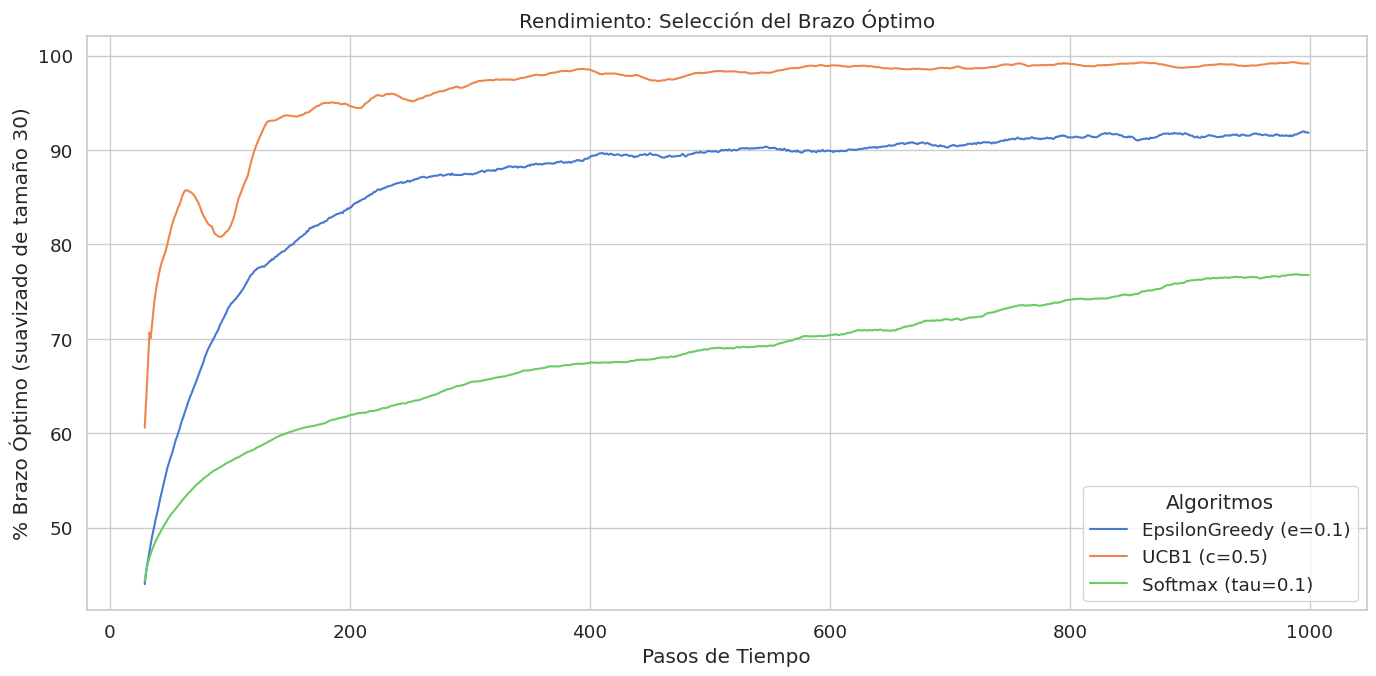
\includegraphics[width=0.9\linewidth]{images/bernouilli_standard.png}
    \caption{Selección óptima para brazos de Bernouilli.}
    \label{fig:bernall}
\end{figure}

\vspace{-20pt}

\begin{figure}[H]
    \centering
    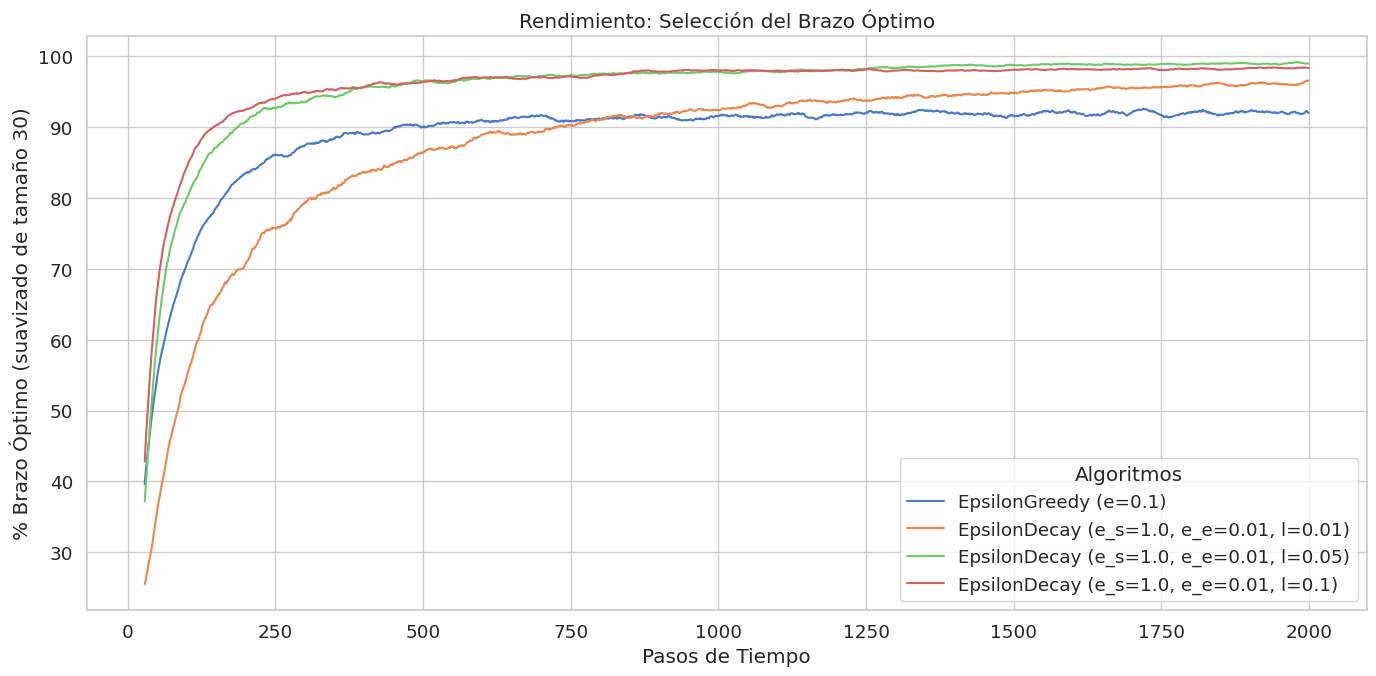
\includegraphics[width=0.8\linewidth]{images/bernouilli_decay.png}
    \caption{Selección óptima para brazos de Bernouilli con Epsilon-Decay.}
    \label{fig:berndecay}
\end{figure}

En el experimento con brazos de probabilidades similares ($p\in[0.4, 0.42, 0.45, 0.48, 0.5]$), la dificultad estadística del problema aumenta: la constante de Lai-Robbins se dispara de $3.12$ a $46.17$. En este contexto, UCB1 mantiene una leve ventaja sobre $\epsilon$-greedy en la tasa de selección óptima, mientras que \textit{Softmax} acumula el mayor arrepentimiento.


\begin{figure}[H]
    \centering
    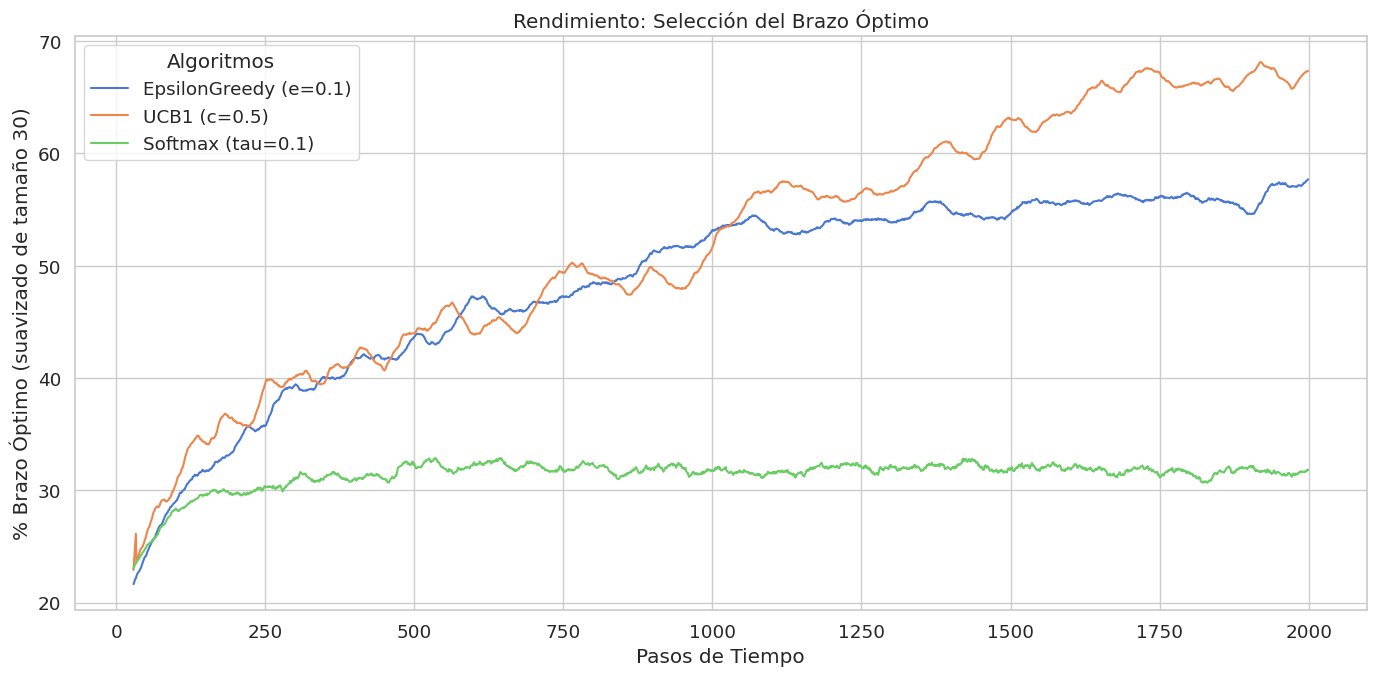
\includegraphics[width=0.9\linewidth]{images/bernouilli_dificil.png}
    \caption{Selección óptima en brazos de Bernouilli similares.}
    \label{fig:bernoulli_dificil}
\end{figure}

\vspace{-20pt}

\subsection{Bandido Binomial}

\subsubsection*{Configuración experimental}
Se modela un bandido de 10 brazos con recompensas de distribución Binomial de $n=10$ ensayos y probabilidades de éxito equiespaciadas en el intervalo $[0.1, 0.9]$, de modo que el brazo óptimo tiene $p=0.9$. Dado que las recompensas se normalizan dividiendo por $n$, el valor esperado de cada brazo coincide directamente con su probabilidad de éxito. Las recompensas son discretas (enteros en $\{0,\dots,n\}$ normalizados a $[0,1]$). Para evaluar los algoritmos ($\epsilon$-\textit{greedy}, UCB1 y \textit{Softmax}), se simulan 1000 iteraciones promediadas sobre 500 ejecuciones independientes. Se utiliza una semilla fija para asegurar la reproducibilidad del experimento.

\subsubsection*{Resultados}

\begin{table}[H]
\centering
\begin{tabular}{|l|c|c|}
\hline
\textbf{Algoritmo} & \textbf{\textit{Regret} Final} & \textbf{\% Sel. Óptima} \\ \hline
$\epsilon$-\textit{greedy} (Decay) & 25.50 & 95.80\% \\ \hline
UCB1 ($c=0.5$) & 37.86 & 94.80\% \\ \hline
\textit{Softmax} ($\tau=0.1$) & 100.18 & 48.60\% \\ \hline
\end{tabular}
\caption{Desempeño promedio en el bandido Binomial.}
\label{tab:resultados_binomial}
\end{table}

\vspace{-20pt}

\subsubsection*{Análisis}

\begin{itemize}
    \item \textbf{Familia $\epsilon$-\textit{greedy}}. Los agentes con $\epsilon$ pequeño ($0.01$) mejoran progresivamente pero de forma lenta, mientras que $\epsilon=0.1$ ofrece el mejor equilibrio entre exploración y explotación dentro de los métodos estáticos. Sin embargo, incluso en este caso el \textit{regret} sigue creciendo linealmente, penalizado por la exploración permanentemente. La variante con decaimiento resuelve esta limitación logrando el menor arrepentimiento acumulado ($\approx 25.50$) y la mayor tasa de selección óptima ($95.80$\%).
\end{itemize}

\begin{figure}[H]
    \centering
    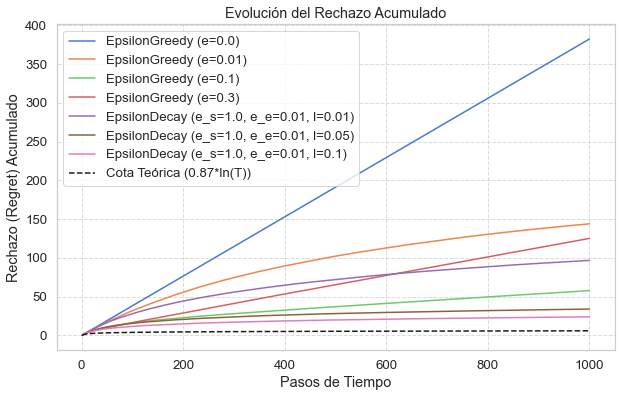
\includegraphics[width=0.80\linewidth]{images/binomial/binom_eps_regret.png}
    \caption{Rechazo acumulado en bandido binomial con $\epsilon$-\textit{greedy}.}
    \label{fig:regret-binom-eps}
\end{figure}


\begin{itemize}
    \item \textbf{Familia UCB}. Los agentes UCB demuestran una solidez notable y una menor sensibilidad a la calibración del parámetro $c$ que $\epsilon$-\textit{greedy} con respecto a $\epsilon$. En contraste con los métodos $\epsilon$-\textit{greedy}, UCB presenta una convergencia con crecimiento logarítmico del arrepentimiento. El valor $c=0.5$ resulta ser el más eficiente en este entorno, alcanzando valores cercanos al óptimo rápidamente y superando el $90$\% de selección óptima al final del horizonte. Valores más altos de $c$ introducen un exceso de exploración que retrasa la convergencia sin beneficio apreciable.
\end{itemize}

\begin{figure}[H]
    \centering
    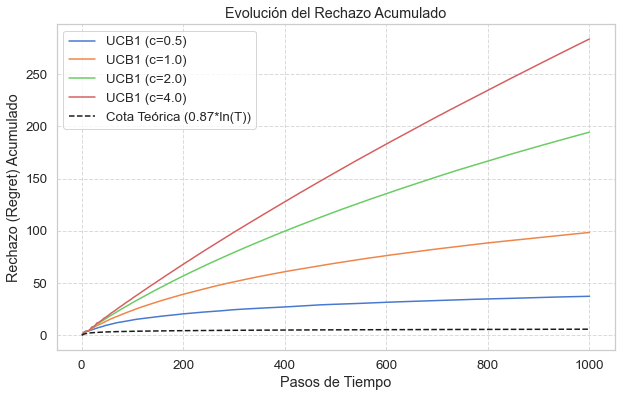
\includegraphics[width=0.80\linewidth]{images/binomial/binom_ucb_regret.png}
    \caption{Rechazo acumulado en bandido binomial con UCB.}
    \label{fig:regret-binom-ucb}
\end{figure}

\begin{itemize}
    \item \textbf{Familia \textit{Softmax}}. Con $\tau=0.1$, \textit{Softmax} logra la mayor velocidad de subida inicial entre todos los algoritmos, pero se estanca entorno al $48.60$\% de selección óptima. Los valores $\tau=0.5$ y $\tau=1.0$ presentan incluso peores resultados por exceso de exploración, mientras que $\tau=0.01$ colapsa de forma casi determinista desde el inicio al igual que $\epsilon$-\textit{greedy} con $\epsilon=0$.
\end{itemize}

\begin{figure}[H]
    \centering
    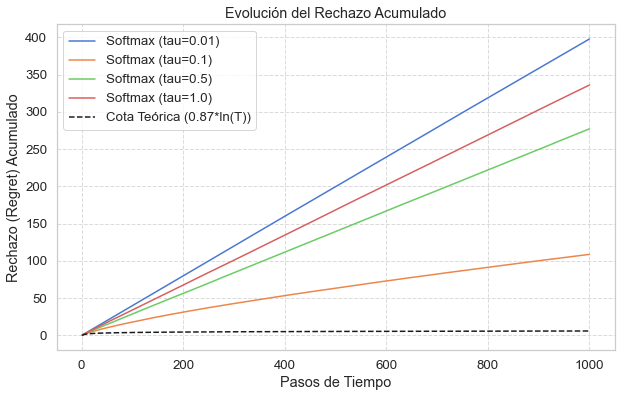
\includegraphics[width=0.80\linewidth]{images/binomial/binom_soft_regret.png}
    \caption{Rechazo acumulado en bandido binomial con \textit{Softmax}.}
    \label{fig:regret-binom-soft}
\end{figure}

\begin{figure}[H]
    \centering
    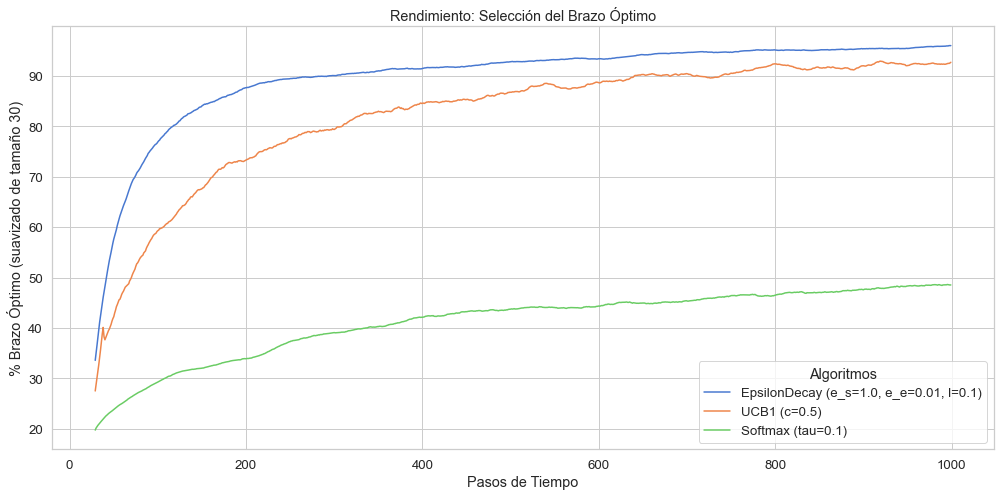
\includegraphics[width=0.8\linewidth]{images/binomial/binom_comp_seleccion.png}
    \caption{Tasa de selección del brazo óptimo en los mejores agentes de cada familia para el bandido binomial.}
    \label{fig:tasa-binom}
\end{figure}


\subsection{Bandido normal}

\subsubsection*{Configuración experimental}

Se utilizan dos bandidos con distribuciones normales con medias $\mu_a\in(0,10)$ y que difieren únicamente en su desviación típica: el  \textbf{bandido sencillo} con $\sigma=1$ (un 10\% del rango de medias) y el \textbf{bandido complejo} con $\sigma=5$ (un 50\% del rango de medias). Nuestra hipótesis es que una mayor varianza ralentizará el aprendizaje y confundirá a los agentes, dado que las distribuciones de recompensa de los brazos se solaparán en mayor medida. Para garantizar la solidez estocástica, el desempeño de los algoritmos se evalúa a lo largo de un horizonte de 1000 iteraciones, promediado sobre 500 ejecuciones independientes. Se prueban variantes de las tres familias de algoritmos con parámetros que favorecen en mayor y menor medida la exploración. 

Cabe destacar que para la familia \textit{Softmax} se han utilizado temperaturas en el rango $\tau\in[0.5,5]$ en lugar del valor $\tau=0.1$ usado en bandidos anteriores. Esto se debe a que, con recompensas en el rango $(0,10)$, valores de $\tau$ pequeños provocan desbordamientos numéricos en el cálculo de las exponenciales ($e^{9/0.1} \gg 2^{63}$).

\subsubsection*{Resultados}

\begin{table}[H]
\centering
\renewcommand{\arraystretch}{1.5} % Ajusta el espaciado vertical para que se vea como en la imagen
\setlength{\tabcolsep}{3pt}      % Ajusta el espacio horizontal entre columnas para que quepa en la columna

\begin{scriptsize} % Tamaño de fuente reducido para asegurar que quepa
\begin{tabular}{l c c c c}
\hline
\textbf{Algoritmo} & \textbf{\textit{Regret}} & \textbf{\% Óptima} & \textbf{\textit{Regret}} & \textbf{\% Óptima} \\ 
 & \textbf{(sencillo)} & \textbf{(sencillo)} & \textbf{(complejo)} & \textbf{(complejo)} \\ 
\hline
$\epsilon$-Greedy ($\epsilon=0.1$) & $\sim$180 & $\sim$75 \% & $\sim$500 & $\sim$55 \% \\ 
\hline
$\epsilon$-Decay ($\lambda=0.01$) & $\sim$260 & $\sim$89 \% & $\sim$480 & $\sim$70 \% \\ 
\hline
$\epsilon$-Decay ($\lambda=0.1$) & $\sim$110 & $\sim$72 \% & $\sim$490 & $\sim$65 \% \\ 
\hline
UCB1 ($c=1$) & $\sim$60 & $>90$ \% & $\sim$420 & $<60$ \% \\ 
\hline
UCB1 ($c=5$) & $\sim$200 & $\sim$65 \% & $\sim$350 & $\sim$85 \% \\ 
\hline
Softmax ($\tau=1$) & $>400$ & $\sim$46 \% & $>500$ & $\sim$43 \% \\ 
\hline
\end{tabular}
\end{scriptsize}

\caption{Desempeño final promedio de los algoritmos en el bandido Normal (valores aproximados en la iteración 1000).}
\vspace{-20pt}
\end{table}


\subsubsection*{Análisis}

\begin{itemize}
    \item \textbf{Familia $\epsilon$-\textit{greedy}} Los algoritmos con exploración baja ($\epsilon=0.005, 0.01$) y decaimiento lento ($\lambda = 0.01$) son los que mayor arrepentimiento acumulan en las primeras iteraciones, sin identificar el brazo óptimo de forma consistente, llegando a tasas inferiores al 60\% en el bandido sencillo y al 50\% en el complejo. El mecanismo de decaimiento mejora notablemente los resultados: un decaimiento rápido ($\lambda = 0.1$) minimiza el arrepentimiento acumulado en el bandido sencillo ($\approx 110 puntos$), mientras que un decaimiento lento ($\lambda=0.01$) alcanza la mayor tasa de selección óptima a largo plazo ($\approx89$\%), a costa de acumular más arrepentimiento en las fases iniciales.

    \item \textbf{Familia UCB}. Los agentes UCB obtienen en general los mejores resultados, pero demuestran una notable sensibilidad a la varianza del problema. En el bandido sencillo, UCB con $c=1$ se consolida como el ganador indiscutible en todas las métricas: supera el 90\% de selección óptima y acumula el menor arrepentimiento, siguiendo de cerca la cota teórica de Lai-Robbins. Sin embargo, en el bandido complejo este mismo agente se estanca entorno a la iteración 200 y no supera el 60\% de selección óptima, confundiendo el brazo óptimo con el segundo mejor (cuyas medias difieren en solo $0.60$ puntos). En este escenario, UCB con $c=5$ se impone claramente: es el único agente que alcanza el $85$\% de selección óptima y cuya curva de arrepentimiento presenta un punto de inflexión visible alrededor de la iteración 200, siendo el único que no se comporta como una función lineal al final del horizonte.
\end{itemize}

\begin{figure}[H]
    \centering
    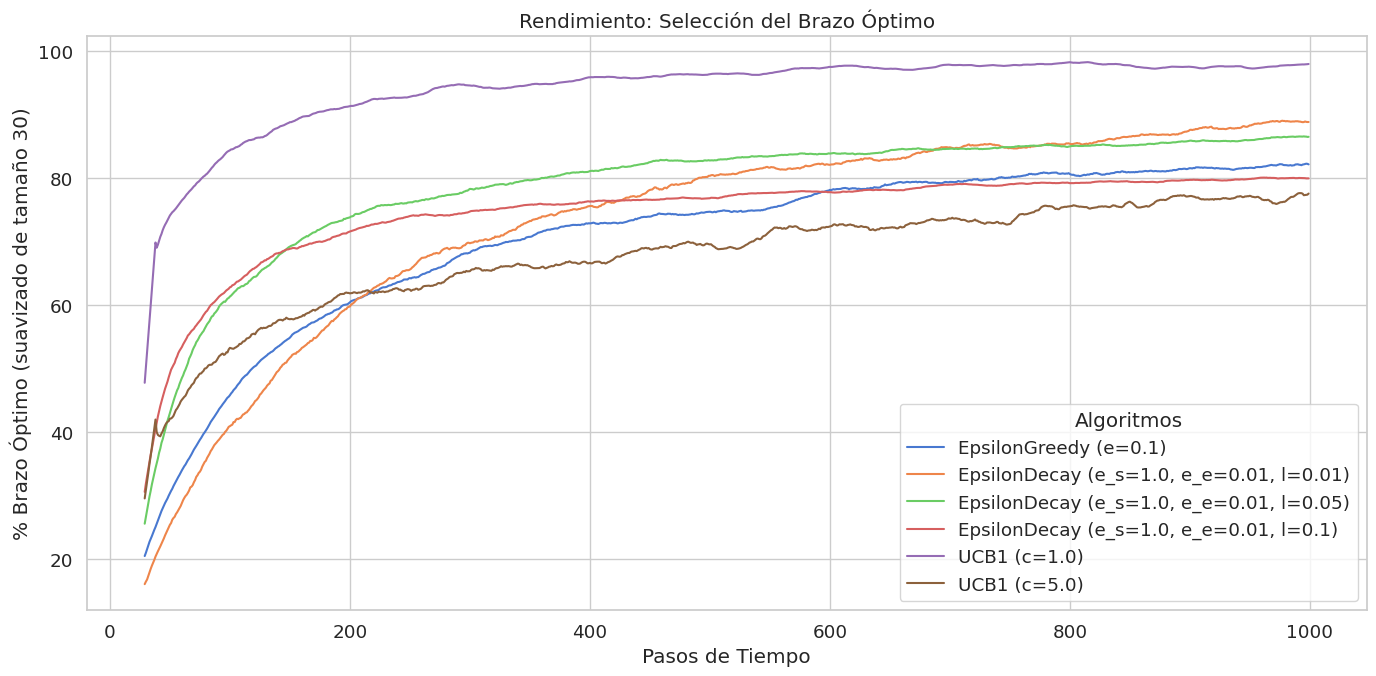
\includegraphics[width=0.8\linewidth]{images/normal/brazo_sencillo.png}
    \caption{Selección del brazo óptimo en el bandido sencillo.}
    \label{fig:tasa-normal-sencillo}
\end{figure}

\begin{figure}[H]
    \centering
    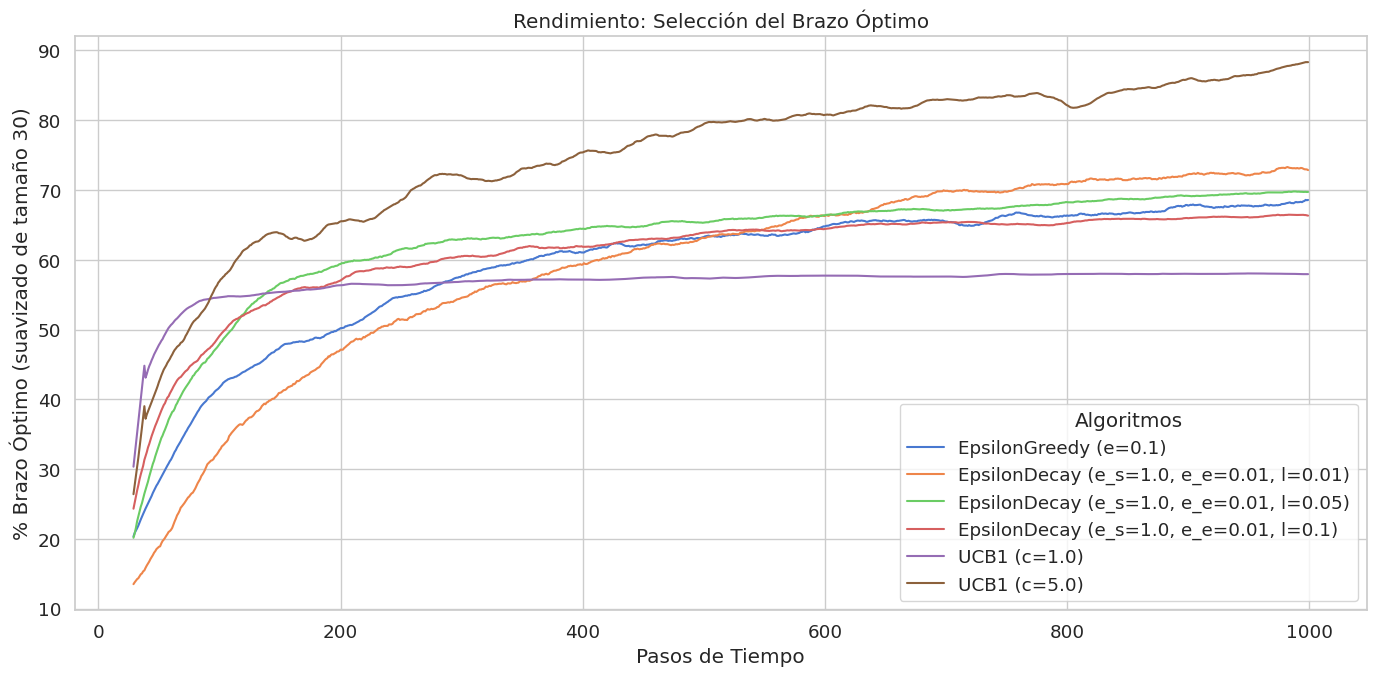
\includegraphics[width=0.8\linewidth]{images/normal/brazo_complejo.png}
    \caption{Selección del brazo óptimo en el bandido complejo.}
    \label{fig:tasa-normal-complejo}
\end{figure}

\begin{figure}[H]
    \centering
    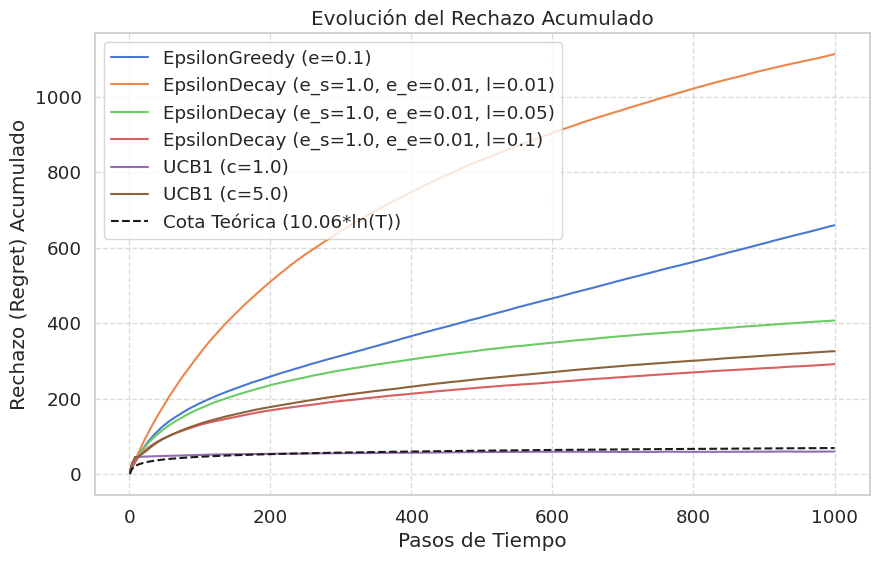
\includegraphics[width=0.8\linewidth]{images/normal/fig_1_5_sencillo_regret.png}
    \caption{\textit{Regret} acumulado en el bandido sencillo.}
    \label{fig:arrepentimiento-normal-sencillo}
\end{figure}

\begin{figure}[H]
    \centering
    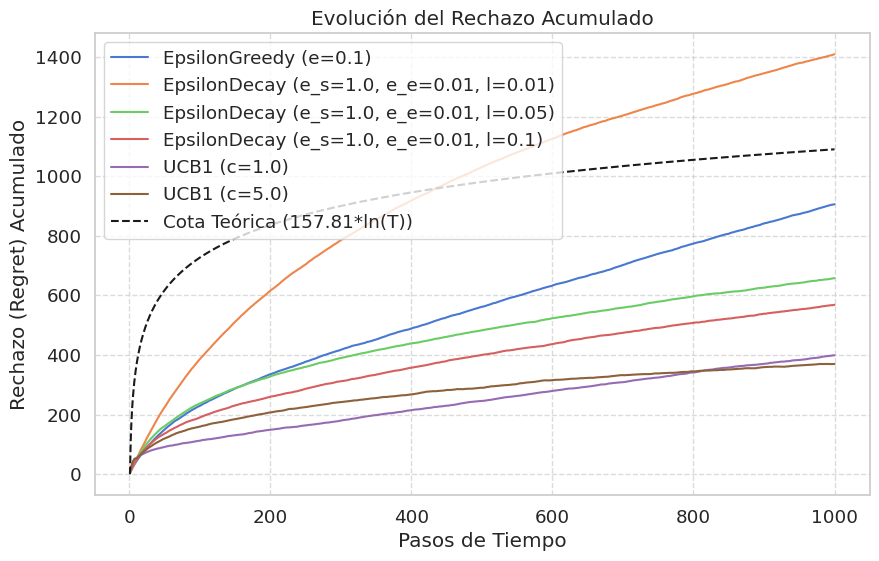
\includegraphics[width=0.8\linewidth]{images/normal/fig_1_5_complejo_regret.png}
    \caption{\textit{Regret} acumulado en el bandido complejo.}
    \label{fig:arrepentimiento-normal-complejo}
\end{figure}

\begin{itemize}
    \item \textbf{Familia \textit{Softmax}}. Es la perdedora con amplia diferencia. El mejor agente ($\tau=1$) es el único que no padece estancamiento temprano y mantiene una tendencia creciente en la iteración 1000, pero su tasa de selección óptima no supera el $46$\% en el bandido sencillo ni el $43$\% en el complejo. Los agentes con temperatura alta ($\tau\geq 2$) adoptan un comportamiento plenamente explotador con tasa de acierto por debajo del $40$\%, mientras que el más explorador ($\tau=0.5$) acumula un arrepentimiento que sigue una tendencia lineal sin signo de convergencia.
\end{itemize}

\begin{figure}[H]
    \centering
    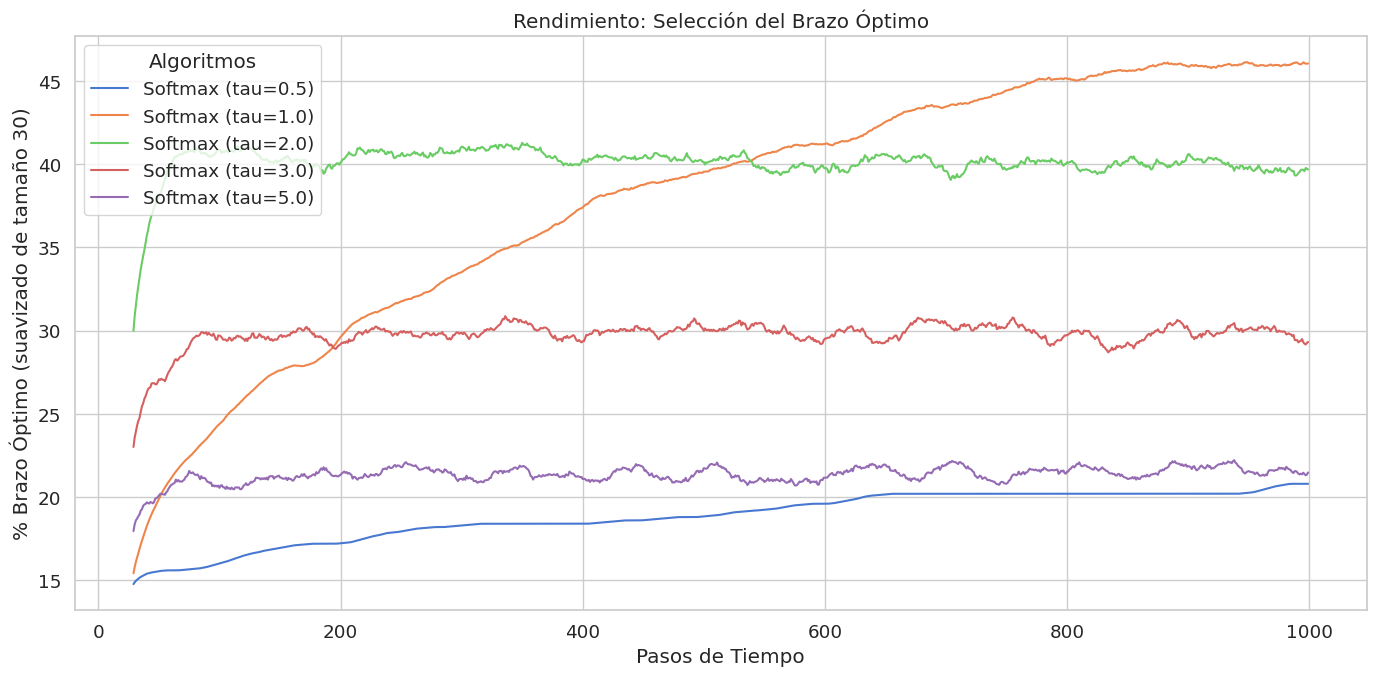
\includegraphics[width=0.8\linewidth]{images/normal/softmax-tasa.png}
    \caption{Tasa de selección del brazo óptimo en el bandido sencillo con estrategias \textit{Softmax}.}
    \label{fig:tasa-normal-softmax}
\end{figure}

\begin{figure}[H]
    \centering
    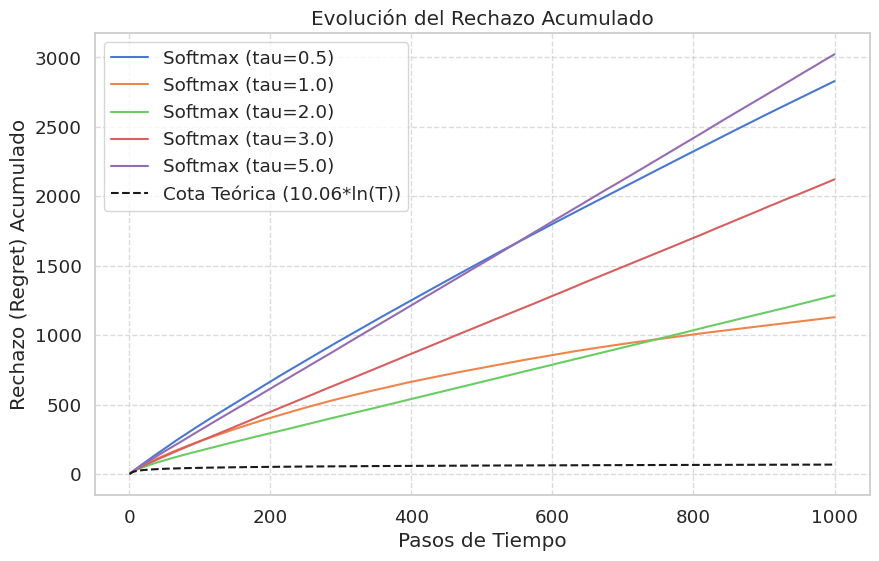
\includegraphics[width=0.8\linewidth]{images/normal/softmax-arrepentimiento.png}
    \caption{Arrepentimiento acumulado en el bandido sencillo con estrategias \textit{Softmax}.}
    \label{fig:arrepentimiento-normal-complejo}
\end{figure}

%%%%%%%%%%%%%%%%%%%%%%%%%%%%%%%%%%%%%%%%%%%%%%%%%%%%%%%%%%%%%
%%%%%%%%%%%%%%%%%%%%%%%%%%%%%%%%%%%%%%%%%%%%%%%%%%%%%%%%%%%%%   
\section{Conclusiones}

A lo largo de este capítulo hemos evaluado tres familias de algoritmos sobre tres tipos de bandidos con distribuciones subyacentes distintas: Bernoulli, binomial y normal. Los resultados permiten extraer conclusiones tanto sobre el comportamiento individual de cada familia como sobre la influencia de la distribución de recompensas en la elección del algoritmo óptimo.

En primer lugar, concluimos que el tipo de distribución tiene un impacto directo y significativo en el rendimiento de los algoritmos. En el bandido de Bernoulli, las recompensas binarias ofrecen una señal clara y de baja varianza, lo que facilita la identificación del brazo óptimo: UCB1 con $c=0.5$ alcanza un 98\% de selección óptima y un \textit{regret} de solo $13.23$. En el bandido binomial, la naturaleza discreta de las recompensas introduce mayor ruido, y Softmax colapsa completamente. En el bandido normal, la varianza es el factor determinante: con $\sigma=1$, UCB1 con $c=1$ domina con un \textit{regret} de $\approx 60$ y más del $90$\% de selección óptima; con $\sigma=5$, ese mismo agente se estanca por debajo del 60\% y es UCB con $c=5$ quien toma el relevo con un $85\%$ de selección óptima y menor arrepentimiento acumulado ($\approx350$). En resumen, a mayor varianza o complejidad en la distribución, más costoso es el proceso de aprendizaje y más necesaria es una exploración elevada. La tabla~\ref{tab:res_t_bandidos} siguiente sintetiza los ganadores por escenario.

\begin{table}
\centering
\renewcommand{\arraystretch}{2} % Aumentamos el espaciado para igualar el estilo visual
\setlength{\tabcolsep}{10pt}    % Espaciado horizontal entre columnas

\begin{scriptsize}
\begin{tabular}{l l l}
\hline
\textbf{Bandido} & \textbf{Ganador (\textit{regret})} & \textbf{Ganador (\% óptima)} \\ 
\hline
Bernoulli & UCB1 ($c = 0.5$) & UCB1 ($c = 0.5$) \\ 
\hline
Binomial & $\epsilon$-Decay ($\lambda = 0.1$) & $\epsilon$-Decay ($\lambda = 0.1$) \\ 
\hline
Normal ($\sigma = 1$) & UCB1 ($c = 1$) & UCB1 ($c = 1$) \\ 
\hline
Normal ($\sigma = 5$) & UCB1 ($c = 5$) & UCB1 ($c = 5$) \\ 
\hline
\end{tabular}
\end{scriptsize}
\caption{Resultados según el tipo de bandido.}
\label{tab:res_t_bandidos}
\end{table}

La elección del algoritmo debe también considerar el horizonte de tiempo disponible. En horizontes cortos, UCB es la opción más clara: su convergencia es rápida y sus exploraciones son mucho más eficientes que las de $\epsilon$-\textit{greedy}. En horizontes largos, la ventaja de UCB se diluye y $\epsilon$-\textit{greedy} con decaimiento se convierte en una alternativa competitiva, especialmente en problemas de alta varianza donde el parámetro $c$ de UCB es difícil de calibrar. \textit{Softmax}, según nuestro estudio, no es recomendable en ningún horizonte temporal sin un proceso de ajuste previo exhaustivo.

Este estudio presenta varias limitaciones que abren líneas de trabajo futuras de interés. En primer lugar, todos los experimentos se han realizado con un número fijo de brazos. Variar $K$ permitiría estudiar cómo escala el coste de exploración con la dimensionalidad del problema. En segundo lugar, hemos evaluado cada familia sobre un único tipo de bandido a la vez. Un análisis con distribuciones mixtas acercaría al experimento a escenarios reales. En tercer lugar, quedan fuera del estudio técnicas de mayor sofisticación teórica como el muestreo de Thompson \cite{thompson1933}, que ha demostrado resultados competitivos con UCB en la literatura \cite{russo2018}, o métodos bayesianos que actualicen distribuciones de probabilidad completas sobre los brazos en lugar de simples estimaciones de media. Finalmente, sería interesante estudiar la robustez de los algoritmos ante bandidos no estacionarios, donde las distribuciones de recompensa cambian paulatinamente a lo largo del tiempo, escenario en el que $\epsilon$-\textit{greedy} con decaimiento podría verse especialmente perjudicado. 